%%%% Better Poster latex template example v1.0 (2019/04/04)
%%%% GNU General Public License v3.0
%%%% Rafael Bailo
%%%% https://github.com/rafaelbailo/betterposter-latex-template
%%%% 
%%%% Original design from Mike Morrison
%%%% https://twitter.com/mikemorrison

\documentclass[a0paper,fleqn]{betterposter}
\graphicspath{{images/}}
\usepackage{hyperref}
\hypersetup{
    colorlinks=true,
    linkcolor=blue,
    filecolor=magenta,      
    urlcolor=cyan,
}
 
\urlstyle{same}

%%%% Uncomment the following commands to customise the format

%% Setting the width of columns
% Left column
%\setlength{\leftbarwidth}{0.25\paperwidth}
% Right column
%\setlength{\rightbarwidth}{0.25\paperwidth}

%% Setting the column margins
% Horizontal margin
%\setlength{\columnmarginvertical}{0.05\paperheight}
% Vertical margin
%\setlength{\columnmarginhorizontal}{0.05\paperheight}
% Horizontal margin for the main column
%\setlength{\maincolumnmarginvertical}{0.15\paperheight}
% Vertical margin for the main column
%\setlength{\maincolumnmarginhorizontal}{0.15\paperheight}

%% Changing font sizes
% Text font
%\renewcommand{\fontsizestandard}{\fontsize{28}{35} \selectfont}
% Main column font
\renewcommand{\fontsizemain}{\fontsize{64}{64} \selectfont}
% Title font
%\renewcommand{\fontsizetitle}{\fontsize{28}{35} \selectfont}
% Author font
%\renewcommand{\fontsizeauthor}{\fontsize{28}{35} \selectfont}
% Section font
%\renewcommand{\fontsizesection}{\fontsize{28}{35} \selectfont}

%% Changing font sizes for a specific text segment
% Place the text inside brackets:
% {\fontsize{28}{35} \selectfont Your text goes here}

%% Changing colours
% Background of side columns
%\renewcommand{\columnbackgroundcolor}{black}
% Font of side columns
%\renewcommand{\columnfontcolor}{gray}
% Background of main column
%\renewcommand{\maincolumnbackgroundcolor}{empirical}
%\renewcommand{\maincolumnbackgroundcolor}{theory}
%\renewcommand{\maincolumnbackgroundcolor}{methods}
%\renewcommand{\maincolumnbackgroundcolor}{intervention}
% Font of main column
%\renewcommand{\maincolumnfontcolor}{gray}

\usepackage[UKenglish]{babel}% http://ctan.org/pkg/babel

\begin{document}	
\betterposter{
%%%%%%%% MAIN COLUMN

\maincolumn{
%%%% Main space

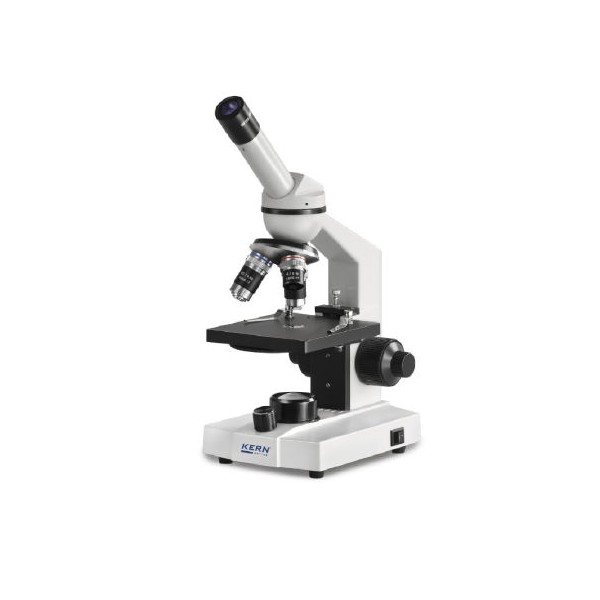
\includegraphics[width=4in]{light} 
Light Microscope:\\
\begin{itemize}
\item Use light to provide magnification.
\item Image is coloured.
\item Controls image formation via glass lenses.
\item No radiation risk.
\item \textbf{Magnification} from 500x to 1500x.
\item The \textbf{specimen} can be dead or alive.
\item It is used for the study of detailed gross internal structure.
\item No \textbf{filament} is used.

\end{itemize}

\bigskip
\bigskip
\bigskip
\bigskip
\bigskip
\bigskip

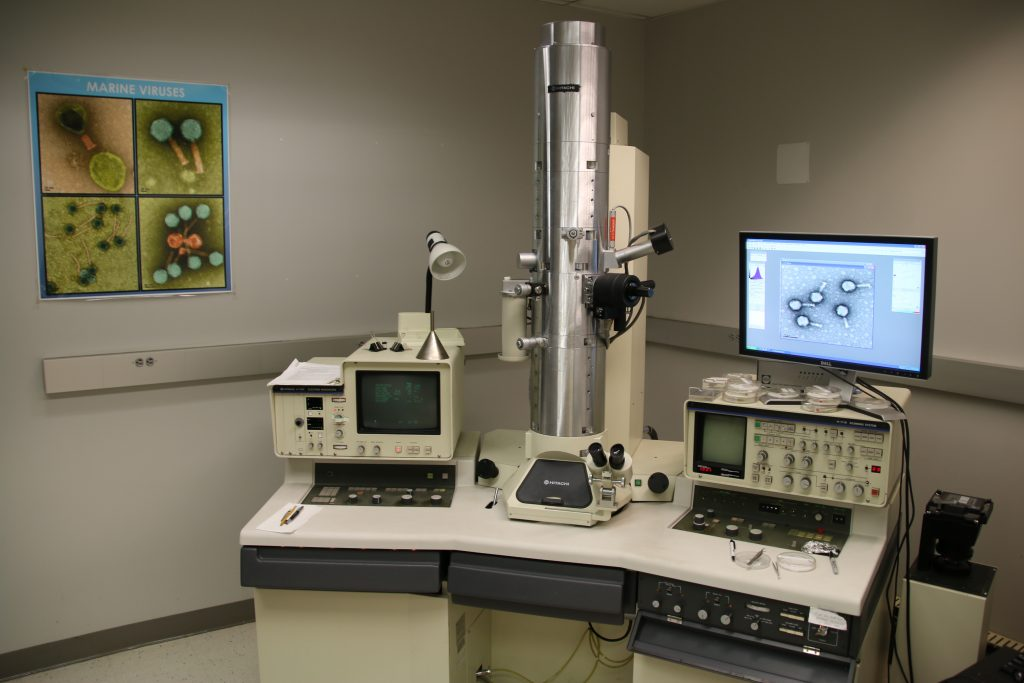
\includegraphics[width=5in]{electron} Electron Microscope:\\
\begin{itemize}
\item Use beams of electrons to work.
\item Image is in black and white.
\item Beams of electrons can be focused using electromagnets.
\item Risk of radiation leakage.
\item Magnification of 100000x to 300000x.
\item Specimen must be dead or dried.
\item Used for external surface, ultra structure of cell and very small organisms. 
\item A tungsten filament is used to produce electrons.
\end{itemize}


}{
%%%% Bottom space

%% QR code
%\qrcode{qrcode}{smartphoneWhite}{
%\textbf{Take a picture} to
%\\download the full paper
%}

% Smartphone icon
% Author: Freepik
% Retrieved from: https://www.flaticon.com/free-icon/smartphone_65680

%% Compact QR code (comment the previous command and uncomment this one to switch)
%\compactqrcode{img/qrcode}{
%\textbf{Take a picture} to
%\\download the full paper
%}

}

}{
%%%%%%%% LEFT COLUMN

\title{Electron and Light microscopes comparison}
\author{Max Sepulveda}
\institution{LVS Ascot}

\section{Introduction}
A microscope is an instrument that magnifies objects otherwise too small to be seen, producing an image in which the object appears larger. Most photographs of cells are taken using a microscope, and these pictures can also be called \emph{micrographs}.
\\

Light microscopes use light, electron microscopes use beams of electrons light controls image formation via glass lenses while beams of electrons can be focused using electromagnets this is because electrons have a negative charge

\bigskip
\bigskip
\bigskip
\bigskip
\bigskip
\bigskip

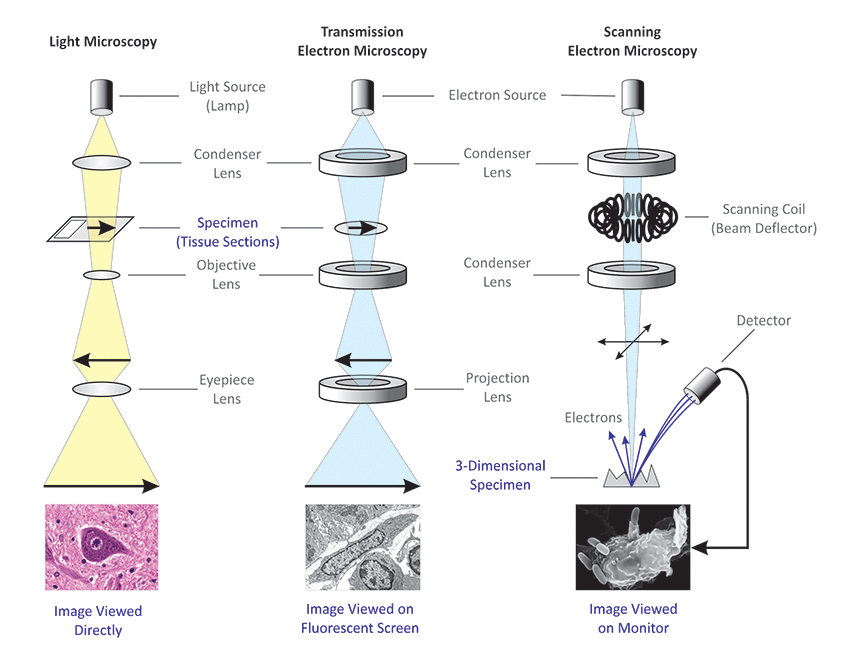
\includegraphics[width=8in]{Light-Microscope-and-Electron-Microscope}


%% This fills the space between the content and the logo
\vfill

}{
%%%%%%%% RIGHT COLUMN

\section{Glosary}
\begin{itemize}

\item Filament: A conducting wire or thread with a high melting point, forming part of an electric bulb or thermionic valve and heated or made incandescent by an electric current.    

\item Specimen: An individual animal, plant, piece of a mineral, etc. used as an example of its species or type for scientific study or display.

\item Magnification: Enlarging the size of an object in an image so you can observe in greater detail.

\end{itemize}

\section{References}
\begin{itemize}
\item Khan Academy, Microscopy.
\Huge \href{https://www.khanacademy.org/science/high-school-biology/hs-cells/hs-introduction-to-cells/a/microscopy}{https://www.khanacademy.org/science/high-school-biology/hs-cells/hs-introduction-to-cells/a/microscopy}
 
\item Microbiology Info, Differences between Light Microscope and Electron Microscope.
\Huge \href{https://microbiologyinfo.com/differences-between-light-microscope-and-electron-microscope/}{https://microbiologyinfo.com/differences-between-light-microscope-and-electron-microscope} 
\end{itemize}
}
\end{document}
